%!TEX root = ../../../FYP_Dissertation.tex


%===============================================================================
% Methodical Accelerator Design
%===============================================================================

\subsection{Lua}
\label{Subsec:Lua}

\begin{wrapfigure}{R}{0.3\textwidth}
    \centering
	
\includegraphics[width=0.25\textwidth]{./Images/Lua.eps}
    % \caption{MAD-NG application}
    \label{fig:lua-logo}
\end{wrapfigure}

Authors claims that Lua is a powerful, efficient, lightweight, embeddable
scripting language. It supports procedural programming, object-oriented
programming, functional programming, data-driven programming, and data
description. Lua combines simple procedural syntax with powerful data description
constructs based on associative arrays and extensible semantics. Lua is
dynamically typed, runs by interpreting bytecode with a register-based virtual
machine, and has automatic memory management with incremental garbage collection.
It has been designed, implemented, and maintained by a team at \emph{PUC-Rio}
(See official website for more info \cite{lua}).

%===============================================================================
% Methodical Accelerator Design
%===============================================================================

\subsection{LuaJIT overview}
\label{Subsec:LuaJIT-overview}

LuaJIT is a Just-In-Time Compiler (JIT) for the Lua programming language. It as
been developed by Mike Pall since 2005. As mentioned on the official website
\cite{luajit-site}, it's widely considered to be one of the fastest dynamic
language implementations. It has outperformed other dynamic languages on many
cross-language benchmarks. This section will try to briefly present LuaJIT
capabilities and how it is arranged internally. For each part a link to the
section providing more details will be provided. Figure \ref{fig:luajit-internal}
depicts a schematic view of LuaJIT internals.

\begin{figure}[H]
    \centering
	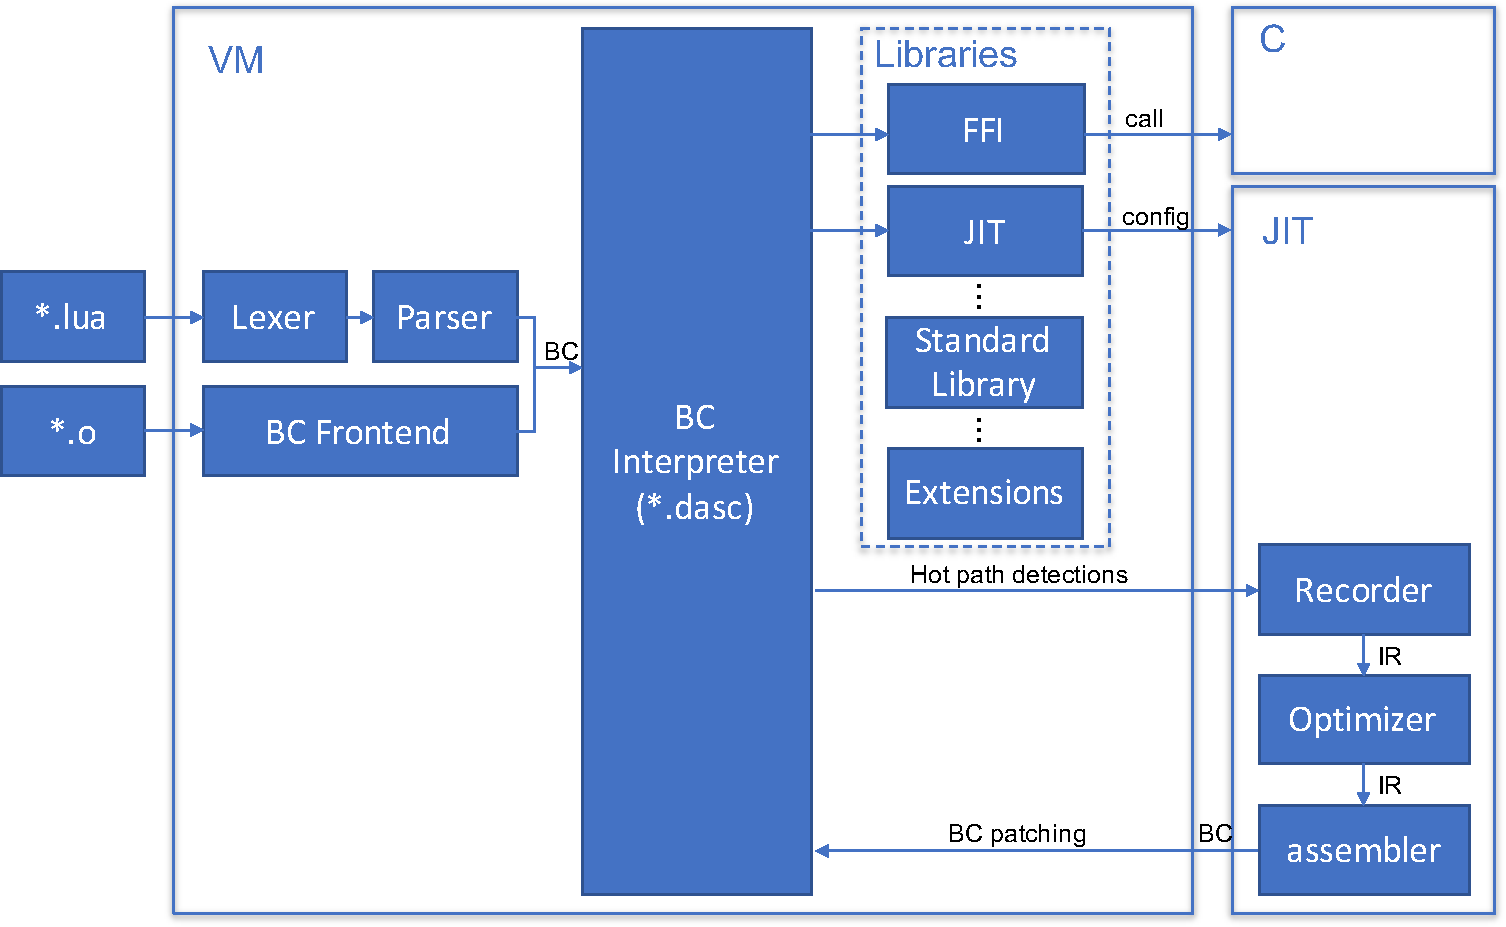
\includegraphics[width=\textwidth]{./Images/LuaJIT.pdf}
    \caption{Schematic view of LuaJIT internals}
    \label{fig:luajit-internal}
\end{figure}{}

First you need to provide luaJIT, files to execute. It accepts two types of input,
text files containing lua code or already converted object files. Lua files are
first read by the \emph{Lexer} \ref{Subsec:Lexer} and \emph{Parser} \ref{Subsec:Parser} and
converted in LuaJIT's bytecode instructions (BC). The other possibility is to provide
object files that contain bytecodes already converted by LuaJIT used for
embedding code in binaries for examples. Those last files are read by the
\emph{bytecode frontend} \ref{Subsec:bc-frontend}.

Once the source code as been converted in bytecode, it is fed to the \emph{bytecode
interpreter} \ref{Sec:BI}. It is the central piece of code written in assembly
that connect every component of luaJIT and is responsible for executing the BC.

There is a certain number of libraries \ref{Sec:Library} packaged will luaJIT, here
to help the BC interpreter to do its work. We will mention a few of them here.
First there is the \emph{FFI} \ref{Sec:FFI} library that allows to directly connect lua
code with c code and c library without lua explicit c interface. The \emph{standard
library} provides a explicit \emph{C} interface to manipulate lua data
(stack, registry, GCObject etc...). Finally, the \emph{JIT} library provides functions
allowing to configure the JIT engine.

The last big part of luaJIT is obviously the \emph{JIT} engine \ref{Chapt:JIT}.
It is actually a tracing JIT that needs to detect \emph{hot path}
\ref{Subsec:hot-path} that would benefit from being compiled. Once such a piece
of bytecode is detected the \emph{recorder} specialize this bytecode with runtime
data and type information and generate an \emph{Intermediate Representation}
equivalent \ref{Subsec:IR}. Then the Optimizer \ref{Sec:TO} modify the IR by
applying a bunch of optimizations on it. Finally, the \emph{assembler} \ref{Sec:TA}
transform the IR into a platform-specific executable binary and the BC that was
detected to be hot is patched to replace his execution to a call to the
corresponding compiled trace.
